%
% File acl2017.tex
%

\documentclass[11pt,a4paper]{article}
\usepackage[hyperref]{acl2017}
\usepackage{times}
\usepackage{url}
\usepackage{latexsym}
\usepackage{times}
\usepackage{url}
\usepackage{amsmath}
\usepackage{breqn}
\usepackage{latexsym}
\usepackage{pgfplotstable}
\usepackage{algorithm2e}
\usepackage{hhline}
\usepackage{multirow}
\usepackage[font=small]{caption}
\usepackage{subcaption}
\usepackage{color}
\usepackage{float}
\usepackage{lipsum,adjustbox}
\usepackage{tikz}
\usepackage{tikz-dependency}
\usetikzlibrary{shapes,fit,calc,er,positioning,intersections,decorations.shapes,mindmap,trees}
\tikzset{decorate sep/.style 2 args={decorate,decoration={shape backgrounds,shape=circle,
      shape size=#1,shape sep=#2}}}
\newcommand{\oa}[1]{\footnote{\color{red} #1}}
\newcommand{\daniel}[1]{\footnote{\color{blue} #1}}
\newcommand{\com}[1]{}
\newcommand{\parser}[1]{TUPA\textsubscript{#1}}
\newcommand{\secref}[1]{Section~\ref{#1}}
\newcommand{\figref}[1]{Figure~\ref{#1}}
\newcommand{\tabref}[1]{Table~\ref{#1}}
\DeclareMathOperator*{\argmin}{argmin}
\DeclareMathOperator*{\argmax}{argmax}
\SetKwRepeat{Do}{do}{while}
\hyphenation{SemEval}
\hyphenation{PARSEVAL}
\hyphenation{DAGParser}
\hyphenation{TurboSemanticParser}
\hyphenation{MaltParser}

%\aclfinalcopy % Uncomment this line for the final submission
%\def\aclpaperid{***} %  Enter the acl Paper ID here

%\setlength\titlebox{5cm}
% You can expand the titlebox if you need extra space
% to show all the authors. Please do not make the titlebox
% smaller than 5cm (the original size); we will check this
% in the camera-ready version and ask you to change it back.

\title{Broad-Coverage Transition-Based UCCA Parsing}

\author{Daniel Hershcovich$^{1,2}$ \And Omri Abend$^2$ \And Ari Rappoport$^2$ \\
  $^1$Edmond and Lily Safra Center for Brain Sciences, Hebrew University of Jerusalem \\
  $^2$School of Computer Science and Engineering, Hebrew University of Jerusalem \\
  \texttt{\{danielh,oabend,arir\}@cs.huji.ac.il}
}

\date{}

\begin{document}
\maketitle

%%%%%%%%%%%%%%%%%%%%%%%%%%%%%%%%%%%%%%%%%%%%%%%%%%%%%%%%%%%%%%%
%%%%%%%%%%%%%%%%%     Abstract     %%%%%%%%%%%%%%%%%%%%%%%%%%%%
%%%%%%%%%%%%%%%%%%%%%%%%%%%%%%%%%%%%%%%%%%%%%%%%%%%%%%%%%%%%%%%
\begin{abstract}
  We present the first parser for UCCA, a
  cross-linguistically applicable framework for semantic
  representation, which builds on extensive
  typological work, and supports rapid annotation.
  UCCA poses a challenge for existing parsing techniques,
  as it exhibits reentrancy (resulting in DAG structures),
  discontinuous structures and non-terminal nodes corresponding
  to complex semantic units. To our knowledge, the conjunction
  of these formal properties is not supported by any existing parser.
  Our transition-based parser, using novel transition set
  and features, has value not just for UCCA parsing:
  its ability to handle more general graph structures will inform
  the development of parsers for other semantic DAG structures, 
  and in languages that frequently use discontinuous structures.
\end{abstract}


%%%%%%%%%%%%%%%%%%%%%%%%%%%%%%%%%%%%%%%%%%%%%%%%%%%%%%%%%%%%%%%
\section{Introduction}\label{sec:introduction}

Universal Conceptual Cognitive Annotation \cite[UCCA,][]{abend2013universal}
is a cross-linguistically applicable semantic representation scheme,
building on the established Basic Linguistic Theory typological framework
\cite{Dixon:10b,Dixon:10a,Dixon:12}, and on Cognitive
Linguistics literature \cite{croft2004cognitive}.
UCCA has demonstrated applicability to multiple languages, including
English, French, German and Czech, support for rapid annotation,
and semantic stability in translation \cite{sulem2015conceptual}.
The scheme has proven useful for machine translation evaluation \cite{birch2016hume},
but its applicability has been so far limited by the absence of a UCCA parser,
a gap this paper addresses.

Formally, a UCCA structure is a DAG (directed acyclic graph)
whose leaves correspond to the tokens of
the text. Nodes (or {\it units}) either correspond to a terminal or
to several sub-units (not necessarily contiguous) jointly viewed as a
single entity according to some semantic or cognitive consideration.
Edges bear a category, indicating the role of the sub-unit in the relation
that the parent represents. \figref{fig:examples} presents a few UCCA-annotated examples.

\begin{figure}[t]
  \begin{subfigure}[t]{.9\columnwidth}
  \parbox{.1\columnwidth}{\caption{}\label{fig:graduation}}
  \parbox{.8\columnwidth}{
  \scalebox{.9}{
  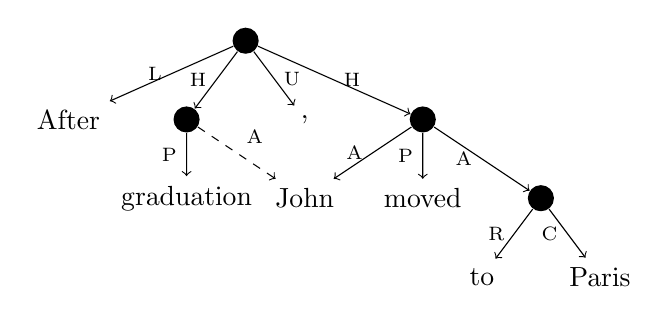
\begin{tikzpicture}[level distance=10mm, ->,
      every circle node/.append style={fill=black}]
    \node (ROOT) [circle] {}
      child {node (After) {After} edge from parent node[left] {\scriptsize L}}
      child {node (graduation) [circle] {}
      {
        child {node {graduation} edge from parent node[left] {\scriptsize P}}
      } edge from parent node[left] {\scriptsize H} }
      child {node {,} edge from parent node[right] {\scriptsize U}}
      child {node (moved) [circle] {}
      {
        child {node (John) {John} edge from parent node[left] {\scriptsize A}}
        child {node {moved} edge from parent node[left] {\scriptsize P}}
        child {node [circle] {}
        {
          child {node {to} edge from parent node[left] {\scriptsize R}}
          child {node {Paris} edge from parent node[left] {\scriptsize C}}
        } edge from parent node[left] {\scriptsize A} }
      } edge from parent node[right] {\scriptsize H} }
      ;
    \draw[dashed,->] (graduation) to node [auto] {\scriptsize A} (John);
  \end{tikzpicture}
  }}
  \end{subfigure}
  \begin{subfigure}[t]{.9\columnwidth}
  \parbox{.1\columnwidth}{\caption{}\label{fig:gave}}
  \hspace{.25\columnwidth}
  \parbox{.55\columnwidth}{
  \scalebox{.9}{
  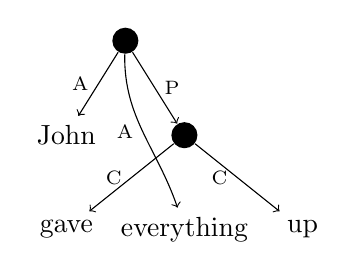
\begin{tikzpicture}[level distance=12mm, ->,
      every node/.append style={midway},
      every circle node/.append style={fill=black}]
    \node (ROOT) [circle] {}
      child {node {John} edge from parent node[left] {\scriptsize A}}
      child {node [circle] {}
      {
      	child {node {gave} edge from parent node[left] {\scriptsize C}}
      	child {node (everything) {everything} edge from parent[white]}
      	child {node {up} edge from parent node[left] {\scriptsize C}}
      } edge from parent node[right] {\scriptsize P} }
      ;
    \draw[bend right,->] (ROOT) to[out=-20, in=180] node [left] {\scriptsize A} (everything);
  \end{tikzpicture}
  }}
  \end{subfigure}
  \begin{subfigure}[t]{.9\columnwidth}
  \parbox{.1\columnwidth}{\caption{}\label{fig:home}}
  \hspace{.1\columnwidth}
  \parbox{.7\columnwidth}{
  \scalebox{.9}{
  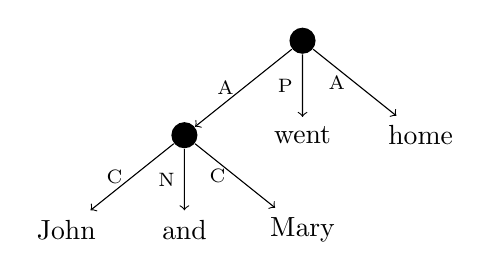
\begin{tikzpicture}[level distance=12mm, ->,
      every node/.append style={midway},
      every circle node/.append style={fill=black}]
    \node (ROOT) [circle] {}
      child {node [circle] {}
      {
        child {node {John} edge from parent node[left] {\scriptsize C}}
        child {node {and} edge from parent node[left] {\scriptsize N}}
        child {node {Mary} edge from parent node[left] {\scriptsize C}}
      } edge from parent node[left] {\scriptsize A} }
      child {node {went} edge from parent node[left] {\scriptsize P}}
      child {node {home} edge from parent node[left] {\scriptsize A}}
      ;
  \end{tikzpicture}
  }}
  \end{subfigure}
  \caption{\label{fig:examples}
    UCCA structures demonstrating three structural properties exhibited by
    the scheme.
    (\subref{fig:graduation}) includes a remote edge (dashed),
    resulting in ``John'' having two parents.
    (\subref{fig:gave}) includes a discontinuous unit (``gave ... up'').
    (\subref{fig:home}) includes a coordination construction (``John and Mary'').
    Legend: $P$ -- process (a scene's main relation), $A$ -- participant,
    $L$ -- inter-scene linker, $H$ -- linked scene, $C$ -- center,
    $R$ -- relator, $N$ -- connector, $U$ -- punctuation, $F$ -- function unit.
    Pre-terminal nodes are omitted for brevity.
  }
\end{figure}

Alongside recent progress in dependency parsing into projective trees
\cite{dyer2015transition,andor2016globally,kiperwasser2016simple},
there is increasing interest in broad-coverage parsing
(see \secref{sec:related_work}),
directed at representations supporting more general structural properties.
One such property is \textbf{reentrancy},
referring to arguments and relations (semantic units) that are shared between predicates.
For instance, in the sentence
``After graduation, John moved to Paris'' (\figref{fig:graduation}),
``John'' is an argument of both ``graduation''
and ``moved'', yielding a UCCA structure that is a DAG rather than a tree.

A second property is \textbf{discontinuity} (similar to \textit{non-projectivity} in bilexical schemes), as in ``John \textit{gave} everything \textit{up}''
(\figref{fig:gave}), where ``gave up'' forms a discontinuous semantic unit.
Discontinuities are pervasive, e.g.,  with multi-word
expressions \cite{schneider2014discriminative}.

Finally, UCCA uses \textbf{non-terminal nodes}
to represent units comprising more than one word.
The use of non-terminal nodes is motivated by constructions that have no clear head, including
coordination structures (e.g., ``\textit{John and Mary} went home''; \figref{fig:home}),
some multi-word expressions (e.g., ``The Haves and the \textit{Have Nots}''),
and prepositional phrases (either the preposition or the head noun can serve as the constituent's head).

No existing parser, to our knowledge, supports the three structural properties described above.
We propose \parser{} (Transition-based UCCA Parser), taking a transition-based approach.
Building on existing knowledge in tackling these three properties
in isolation, we define an extended set of transitions and features
that support reentrancy, discontinuities and non-terminal nodes.

Transition-based techniques are a natural
starting point for UCCA parsing, given the conceptual similarity of UCCA's distinctions,
centered around predicate-argument structures, to distinctions expressed by dependency schemes.
We are further motivated by the strength of transition-based methods
in similar tasks, including syntactic dependency parsing
\cite{dyer2015transition,andor2016globally,kiperwasser2016simple},
dependency graph parsing
\cite{sagae2008shift,ribeyre-villemontedelaclergerie-seddah:2014:SemEval,tokgoz2015transition},
constituency parsing \cite{sagae2005classifier,zhang2009transition,zhu2013fast,maier2015discontinuous,maier-lichte:2016:DiscoNLP},
AMR parsing \cite{wang-xue-pradhan:2015:ACL-IJCNLP,wang2015transition,wang-EtAl:2016:SemEval,dipendra2016neural,goodman2016noise,zhou2016amr,damonte2016incremental}
and CCG parsing \cite{ambati2015incremental,ambati-deoskar-steedman:2016:N16-1},
as well as joint lexical and syntactic parsing
\cite{constant-nivre:2016:P16-1}.
\parser{} mostly builds on recent advances in discontinuous constituency
and dependency graph parsing, and further introduces novel features for UCCA.

We evaluate \parser{} on the available English UCCA corpora, in both
in-domain and out-of-domain settings (\secref{sec:exp_setup}).
As a point of comparison, we assess the ability of existing
parsers to tackle the task, by developing a conversion procedure
from UCCA to bilexical graphs and trees.
Results show superior accuracy for \parser{}, demonstrating the effectiveness of
the presented approach (\secref{sec:results}).
All converters and parsers will be made publicly available upon publication.


%%%%%%%%%%%%%%%%%%%%%%%%%%%%%%%%%%%%%%%%%%%%%%%%%%%%%%%%%%%%%%%
\section{The UCCA Scheme}\label{sec:ucca}

UCCA is a multi-layered representation, each layer corresponding
to a ``module'' of semantic distinctions.
The UCCA \textbf{foundational layer}, which we target in this paper, covers the predicate-argument
structure evoked by predicates of all grammatical categories
(verbal, nominal, adjectival and others), the inter-relations between them,
and other major linguistic phenomena such as coordination and multi-word expressions.

The layer's basic notion is the {\it Scene}, describing a movement, action or state.
Each Scene contains one main relation (marked as either a Process or a State),
as well as one or more Participants.
For example, the sentence ``After graduation, John moved to Paris'' (\figref{fig:graduation})
contains two Scenes, whose main relations are ``graduation'' and ``moved''.
``John'' is a Participant in both Scenes, while ``Paris'' only in the latter.
One incoming edge for each non-root node is marked as \textbf{primary},
and the rest (mostly denoting implied relations) as \textbf{remote} edges.
This distinction is made by the annotator.
The primary edges thus form a tree structure, whereas the remote edges enable reentrancy,
thus forming a DAG.

Further categories account for relations between Scenes and the internal structure of
complex arguments and relations (e.g. coordination; complex
adverbials such as ``very clearly'').
%\footnote{All UCCA-related resources can be found here:
%  \url{http://www.cs.huji.ac.il/~oabend/ucca.html}.}


%%%%%%%%%%%%%%%%%%%%%%%%%%%%%%%%%%%%%%%%%%%%%%%%%%%%%%%%%%%%%%%
\section{Transition-based UCCA Parsing}\label{sec:direct_approach}

We now turn to presenting \parser{},
a transition-based parser supporting the structural properties of UCCA.
Transition-based parsers \cite{Nivre03anefficient} scan the text from start to end,
and create the parse incrementally by applying a \textit{transition}
at each step to the parser state,
defined using three data structures: a buffer $B$ of tokens and nodes to be processed,
a stack $S$ of nodes currently being processed,
and a graph $G=(V,E,\ell)$ of constructed nodes and edges,
where $V$ is the set of \emph{nodes}, $E$ is the set of \emph{edges},
and $\ell : E \to L$ is the \emph{label} function, $L$ being the set of possible labels.
Some of the states are marked as \textit{terminal}, meaning that $G$ is the final output.
A classifier is used at each step to select the next transition based on features
encoding the parser's current state.
During training, an oracle creates training instances for the classifier,
based on gold-standard annotations.

\paragraph{Transition Set.}
Given a sequence of tokens $w_1, \ldots, w_n$, we predict a UCCA graph $G$ over the sequence.
Parsing starts with a single node on the stack (an artificial root node), and the input tokens
in the buffer. The set of transitions is given in \figref{fig:transitions}.
In addition to the standard \textsc{Shift} and \textsc{Reduce} operations, 
we follow previous work in transition-based constituency parsing \cite{sagae2005classifier},
adding the \textsc{Node} transition for creating new non-terminal nodes.
\textsc{Node$_X$} creates a new node on the buffer as a parent of the first element on the stack, with an $X$-labeled edge.


\begin{figure*}
\begin{adjustbox}{width=\textwidth,margin=3pt,frame}
\begin{tabular}{llll|l|llllc|c}
\multicolumn{4}{c|}{\textbf{\small Before Transition}} & \textbf{\small Transition} & \multicolumn{5}{c|}{\textbf{\small After Transition}} & \textbf{\small Condition} \\
\textbf{\footnotesize Stack} & \textbf{\footnotesize Buffer} & \textbf{\footnotesize Nodes} & \textbf{\footnotesize Edges} & & \textbf{\footnotesize Stack} & \textbf{\footnotesize Buffer} & \textbf{\footnotesize Nodes} & \textbf{\footnotesize Edges} & \textbf{\footnotesize Terminal?} & \\
$S$ & $x \;|\; B$ & $V$ & $E$ & \textsc{Shift} & $S \;|\; x$ & $B$ & $V$ & $E$ & $-$ & \\
$S \;|\; x$ & $B$ & $V$ & $E$ & \textsc{Reduce} & $S$ & $B$ & $V$ & $E$ & $-$ & \\
$S \;|\; x$ & $B$ & $V$ & $E$ & \textsc{Node$_X$} & $S \;|\; x$ & $y \;|\; B$ & $V \cup \{ y \}$ & $E \cup \{ (y,x)_X \}$ & $-$ &
$x \neq \mathrm{root}$ \\
$S \;|\; y,x$ & $B$ & $V$ & $E$ & \textsc{Left-Edge$_X$} & $S \;|\; y,x$ & $B$ & $V$ & $E \cup \{ (x,y)_X \}$ & $-$ &
\multirow{4}{50pt}{\vspace{-5mm}\[\left\{\begin{array}{l}
x \not\in w_{1:n},\\
y \neq \mathrm{root},\\
y \not\leadsto_G x
\end{array}\right.\]} \\
$S \;|\; x,y$ & $B$ & $V$ & $E$ & \textsc{Right-Edge$_X$} & $S \;|\; x,y$ & $B$ & $V$ & $E \cup \{ (x,y)_X \}$ & $-$ & \\
$S \;|\; y,x$ & $B$ & $V$ & $E$ & \textsc{Left-Remote$_X$} & $S \;|\; y,x$ & $B$ & $V$ & $E \cup \{ (x,y)_X^* \}$ & $-$ & \\
$S \;|\; x,y$ & $B$ & $V$ & $E$ & \textsc{Right-Remote$_X$} & $S \;|\; x,y$ & $B$ & $V$ & $E \cup \{ (x,y)_X^* \}$ & $-$ & \\
$S \;|\; x,y$ & $B$ & $V$ & $E$ & \textsc{Swap} & $S \;|\; y$ & $x \;|\; B$ & $V$ & $E$ & $-$ &
$\mathrm{i}(x) < \mathrm{i}(y)$ \\
$[\mathrm{root}]$ & $\emptyset$ & $V$ & $E$ & \textsc{Finish} & $\emptyset$ & $\emptyset$ & $V$ & $E$ & $+$ & \\
\end{tabular}
\end{adjustbox}
\caption{\label{fig:transitions}
  The transition set of \parser{}. %Following standard practice,
  We write the stack with its top to the right and the buffer with its head to the left.
  $(\cdot,\cdot)_X$ denotes a primary $X$-labeled edge, and $(\cdot,\cdot)_X^*$ a remote $X$-labeled edge.
  $\mathrm{i}(x)$ is a running index for the created nodes.
  In addition to the specified conditions,
  the prospective child in an \textsc{Edge} transition must not already have a primary parent.
}
\end{figure*}

\textsc{Left-Edge$_X$} and \textsc{Right-Edge$_X$} create a new primary $X$-labeled edge between the first two elements on the stack, where the parent is the left or the right node, respectively.
As a UCCA node may only have one incoming primary edge,
\textsc{Edge} transitions are disallowed if the child node already
has an incoming primary edge.
\textsc{Left-Remote$_X$} and \textsc{Right-Remote$_X$} do not have this restriction,
and the created edge is additionally marked as \textit{remote}.
We distinguish between these two pairs of transitions to allow the parser to create remote edges
without the possibility of producing invalid graphs.
To support the prediction of multiple parents, node and edge transitions
leave the stack unchanged, as in other work on
transition-based dependency graph parsing
\cite{sagae2008shift,ribeyre-villemontedelaclergerie-seddah:2014:SemEval,tokgoz2015transition}.
Once all edges for a node have been created, it is removed from the stack
by applying \textsc{Reduce}.
To handle discontinuous nodes, \textsc{Swap} pops the second
node on the stack and adds it to the top of the buffer, as with the similarly
named transition in previous work \cite{nivre2009non,maier2015discontinuous}.
Finally, \textsc{Finish} pops the root node and marks the state as terminal.

\paragraph{Classifier.}
We experiment with four classifiers.
Our first parser (\parser{Sparse}), following \citet{maier-lichte:2016:DiscoNLP},
uses a linear classifier, with sparse features and
the averaged structured perceptron algorithm for training it
\cite{Coll:04}. We use the \textsc{MinUpdate} procedure \cite{goldberg2011learning}:
a minimum number of updates to a feature has to occur in training for it
to be included in the model.
Our second parser (\parser{Dense}) also uses a linear classifier
trained using averaged structured perceptron, but with dense embedding features (see below).
Our third parser (\parser{MLP} for ``multi-layer perceptron'') uses a feedforward neural network,
similar in architecture to that of \citet{chen2014fast}, with the following modifications:
two hidden layers instead of one, using the ReLU activation function instead of the cube,
and applying dropout after each layer \cite{srivastava2014dropout}.
Our fourth parser (\parser{BiLSTM}) uses a bidirectional LSTM to represent the tokens,
similar to \cite{kiperwasser2016simple}, followed by two feedforward layers similar to \parser{MLP}.

For all classifiers, inference is performed greedily, i.e., without beam search.

\paragraph{Features.}
For the sparse perceptron-based parser (\parser{Sparse}),
we use binary indicator features representing
the words, POS tags, syntactic dependency labels and
existing edge labels related to the top four stack elements and the 
next three buffer elements, in addition to their children and grandchildren in the graph.
We also use bi- and trigram features based on these values \cite{zhang2009transition,zhu2013fast},
features related to discontinuous nodes adopted from \citet{maier2015discontinuous}
(including separating punctuation and gap type),
features representing existing edges and the number of parents and children a node has, following \citet{tokgoz2015transition},
and the past actions performed by the parser.
We also use a novel, UCCA-specific feature:
number of remote children\footnote{See
Appendix~\ref{appendix:features} for a full listing of the feature templates.}.

For the dense perceptron-based (\parser{Dense}) and the NN-based parsers
(\parser{MLP} and \parser{BiLSTM}),
we replace all indicator features by a
concatenation of the vector embeddings of all represented elements:
words, POS tags, syntactic dependency labels, edge labels, punctuation, gap type and parser actions.

Finally, for all classifiers we add another real-valued feature to the input vector,
\textbf{ratio}, corresponding to the ratio between the number of terminals to number of nodes
in the graph $G$.
This novel feature serves as a regularizer for the creation of new nodes,
and should be beneficial for other transition-based constituency parsers too.

\paragraph{Training.}
For training the transition classifiers, we use a dynamic oracle \cite{goldberg2012dynamic},
i.e., an oracle that outputs a set of optimal transitions: when
applied to the current parser state, the gold
standard graph is reachable from the resulting state.
For example, the oracle would predict a \textsc{Node} transition if the stack 
has on its top a parent in the gold graph that has not been created,
but would predict a \textsc{Right-Edge} transition if the second stack
element is a parent of the
first element according to the gold graph and the edge between them has not been created.
The transition predicted by the classifier is deemed correct
and is applied to the parser state to reach the subsequent state,
if the transition is included in the set of optimal transitions.
Otherwise, a random optimal transition is applied,
and for the perceptron-based parser, the classifier's weights are updated according
to the perceptron update rule.

We double the weight updates
for gold \textsc{Swap} transitions to address the sparsity of discontinuous nodes,
as in \citet{maier2015discontinuous}.
POS tags and syntactic dependnecy labels are extracted using spaCy\footnote{\url{https://spacy.io}}
\cite{honnibal-johnson:2015:EMNLP}.
External word embeddings are initialized with
100-dimensional pre-trained word2vec vectors \cite{mikolov2013efficient},
the same ones used by \citet{dyer2015transition}\footnote{
\url{https://github.com/clab/lstm-parser}}.

For the NN classifiers, in addition to the external word embeddings, we use
randomly initialized word embeddings.
For both the dense perceptron and the NN classifiers,
we initialize all other embeddings randomly.
We use the categorical cross-entropy objective function and optimize the
NN classifiers with the Adam optimizer \cite{kingma2014adam}.
We use the DyNet package\footnote{\url{https://github.com/clab/dynet}}
\cite{neubig2017dynet} for implementing the NN classifiers.
Unless otherwise noted, we use the default values provided by the package.
\tabref{table:hyperparameters} lists the hyperparameter values we found by tuning
on the development set.

\begin{table}
\scalebox{.9}{
\begin{tabular}{l|cccc}
& \multicolumn{2}{c|}{\footnotesize Perceptron} & \multicolumn{2}{c}{\footnotesize NN} \\
& Sparse & Dense & MLP & BiLSTM \\
\hline
\multicolumn{4}{l}{\footnotesize Embedding dim.} \\
external word & & 100 & 100 & 100 \\
word & & & 200 & 50 \\
POS tag & & 10 & 10 & 20 \\
syntactic dep. & & 10 & 10 & 20 \\
edge label & & 20 & 10 & 5 \\
punctuation & & 2 & 3 & 2 \\
gap & & 2 & 1 & 3 \\
action & & 5 & 10 & 10 \\
\hline
\multicolumn{4}{l}{\footnotesize Other parameters} \\
MLP \#layers & & & 2 & 2 \\
MLP layer dim. & & & 100 & 200 \\
LSTM \#layers & & & & 2 \\
LSTM layer dim. & & & & 1000 \\
word dropout & & & 0.3 & 0.3 \\
ex. word dropout & & & 0.3 & 0.3 \\
L2 regularizer & & & $10^{-6}$ & $10^{-4}$ \\
dropout & & & 0.1 & 0.5 \\
mini-batch size & & & 1000 & 1000 \\
training iterations & 13 & 11 & 6 & 6 \\
$\textsc{MinUpdate}$ & 5 \\
\end{tabular}
}
\caption{Hyperparameters used for the different classifiers.}
\label{table:hyperparameters}
\end{table}

%%%%%%%%%%%%%%%%%%%%%%%%%%%%%%%%%%%%%%%%%%%%%%%%%%%%%%%%%%%%%%%
\section{Experimental Setup}\label{sec:exp_setup}

\paragraph{Data.}
We conduct our main experiments on the UCCA Wikipedia corpus (henceforth, \textit{Wiki}),
and use the English part of the UCCA \textit{Twenty Thousand Leagues Under the Sea}
English-French parallel corpus (henceforth, \textit{20K Leagues}) as
out-of-domain data.\footnote{\mbox{\url{http://cs.huji.ac.il/~oabend/ucca.html}}}
\tabref{table:data} presents some statistics for the two corpora, demonstrating that while
the \textit{Wiki} corpus is over ten times larger, the overall statistics are
similar.
We use passages of indices up to 676
of the \textit{Wiki} corpus as our training set, passages 688--808 as development set,
and passages 942--1028 as in-domain test set.
While UCCA edges can cross sentence boundaries, we adhere to the common
practice in semantic parsing and train our parsers on individual sentences,
discarding inter-relations between them (0.18\% of the edges).
We also discard linkage nodes and edges (as they often express inter-sentence
relations and are thus mostly redundant when applied at the sentence level)
as well as implicit nodes\footnote{See Appendix~\ref{appendix:extended_ucca}
for details about Linkage and Implicit.}.
In the out-of-domain experiments, we apply the same parsers
(trained on the \textit{Wiki} training set) to the \textit{20K Leagues} corpus
without parameter re-tuning.


\begin{table}
\scalebox{.9}{
\begin{tabular}{l|ccc|c}
& \multicolumn{3}{c|}{Wiki} & 20K \\
& \small Train & \small Dev & \small Test & Leagues \\
\hline
\# passages & 300 & 34 & 33 & 154 \\
\# sentences & 4268 & 454 & 503 & 506 \\
\hline
\# nodes & 298,993 & 33,704 & 35,718 & 29,315 \\
\% terminal & 42.96 & 43.54 & 42.87 & 42.09 \\
\% non-term. & 58.33 & 57.60 & 58.35 & 60.01 \\
\% discont. & 0.54 & 0.53 & 0.44 & 0.81 \\
\% reentrant & 2.38 & 1.88 & 2.15 & 2.03 \\
\hline
\# edges & 287,914 & 32,460 & 34,336 & 27,749 \\
\% primary & 98.25 & 98.75 & 98.74 & 97.73 \\
\% remote & 1.75 & 1.25 & 1.26 & 2.27 \\
\hline
\multicolumn{3}{l}{\footnotesize Average per non-terminal node} \\
\# children & 1.67 & 1.68 & 1.66 & 1.61 
\end{tabular}
}
\caption{Statistics of the \textit{Wiki} and \textit{20K Leagues} UCCA corpora.
All counts exclude the root node, implicit nodes, and linkage nodes and edges.
}
\label{table:data}
\end{table}

\paragraph{Evaluation.}
Since there are no standard evaluation measures for UCCA, we define
two simple measures for comparing such structures.
Assume $G_p=(V_p,E_p,\ell_p)$ and $G_g=(V_g,E_g,\ell_g)$
are the predicted and gold-standard graphs over the same
sequence of terminals $W = \{w_1,\ldots,w_n\}$, respectively.
For an edge $e=(u,v)$ in either graph,
where $u$ is the parent and $v$ is the child, define its yield $y(e) \subseteq W$ as the
set of terminals in $W$ that are descendants of $v$.
Define the set of \textit{mutual edges} between $G_p$ and $G_g$:

\vspace{-.6cm}

{\small
\begin{multline*}
    M(G_p,G_g) = \\
    \left\{(e_1,e_2) \in E_p \times E_g \;|\;
    y(e_1) = y(e_2) \wedge \ell_p(e_1)=\ell_g(e_2)\right\}
\end{multline*}
}

\vspace{-.6cm}

Labeled precision and recall are defined by dividing $|M(G_p,G_g)|$ by $|E_p|$ and $|E_g|$, respectively,
and F-score by taking their harmonic mean.
We report two variants of this measure: one where we consider only primary edges,
and another for remote edges (see \secref{sec:ucca}).
We note that the measure collapses to the standard
PARSEVAL constituency evaluation measure if $G_p$ are $G_g$ are trees.
Punctuation is excluded from the evaluation, but not from the datasets.

\paragraph{Linguistic constructions.}

In addition to the overall evaluation on primary and remote edges,
we perform fine-grained evaluation on various linguistic construction,
which we extract by criteria on UCCA edge labels and POS tags.\footnote{See
Appendix~\ref{appendix:constructions} for a listing of the criteria.}
For each construction, we report the F-score resulting from calculating the
mutual edges only among the edges matching the criterion in each graph.

\begin{figure}[ht]
\centering
\scalebox{.9}{
\begin{dependency}[theme = simple]
\begin{deptext}[column sep=.7em,ampersand replacement=\^]
After \^ graduation \^ , \^ John \^ moved \^ to \^ Paris \\
\end{deptext}
\depedge{2}{1}{L}
\depedge{2}{3}{U}
\depedge[dashed]{2}{4}{A}
\depedge{5}{4}{A}
\depedge{2}{5}{H}
\depedge{7}{6}{R}
\depedge{5}{7}{A}
\end{dependency}
}
\begin{dependency}[theme = simple]
\begin{deptext}[column sep=.7em,ampersand replacement=\^]
John \^ gave \^ everything \^ up \\
\end{deptext}
\depedge{1}{2}{A}
\depedge{3}{2}{A}
\depedge{4}{2}{C}
\end{dependency}
\begin{dependency}[theme = simple]
\begin{deptext}[column sep=.7em,ampersand replacement=\^]
John \^ and \^ Mary \^ went \^ home \\
\end{deptext}
\depedge[edge start x offset=-6pt]{1}{4}{A}
\depedge{2}{1}{N}
\depedge{3}{1}{C}
\depedge{5}{4}{A}
\end{dependency}
\caption{Bilexical approximation for sentences in \figref{fig:examples}.}
\label{fig:bilexical_example}
\end{figure}

\begin{table*}[ht]
\begin{tabular}{l|ccc|ccc||ccc|ccc}
& \multicolumn{6}{c||}{Wiki (in-domain)} & \multicolumn{6}{c}{20K Leagues (out-of-domain)} \\
& \multicolumn{3}{c|}{Primary} & \multicolumn{3}{c||}{Remote}
& \multicolumn{3}{c|}{Primary} & \multicolumn{3}{c}{Remote} \\
& \textbf{LP} & \textbf{LR} & \textbf{LF} & \textbf{LP} & \textbf{LR} & \textbf{LF}
& \textbf{LP} & \textbf{LR} & \textbf{LF} & \textbf{LP} & \textbf{LR} & \textbf{LF} \\
\hline
\multicolumn{4}{l}{\rule{0pt}{2ex} \footnotesize Bilexical Approximation} \\
\small Upper Bound
& \small 94.5 & \small 87.7 & \small 91 & \small 77.3 & \small 46.8 & \small 58.3
& \small 94.8 & \small 88 & \small 91.3 & \small 66.3 & \small 32.3 & \small 43.4 \\
DAGParser
& 61.8 & 55.8 & 58.6 & 9.5 & 0.5 & 1
& 56.4 & 50.6 & 53.4 & -- & 0 & 0 \\
TurboParser
& 57.7 & 46 & 51.2 & 77.8 & 1.8 & 3.7
& 50.3 & 37.7 & 43.1 & 100 & 0.4 & 0.8 \\
\hline
\multicolumn{4}{l}{\rule{0pt}{2ex} \footnotesize Tree Approximation} \\
\small Upper Bound
& \small 100 & \small 100 & \small 100 & & &
& \small 100 & \small 100 & \small 100 \\
\textsc{uparse}
& 60.9 & 61.2 & 6 & & &
& 52.7 & 52.8 & 52.8 \\
\hline
\multicolumn{4}{l}{\rule{0pt}{2ex} \footnotesize Bilexical Tree Approximation} \\
\small Upper Bound
& \small 94.5 & \small 87.7 & \small 91 & & &
& \small 94.8 & \small 88 & \small 91.3 \\
MaltParser
& 62.8 & 57.7 & 60.2 & & &
& 57.8 & 53 & 55.3 \\
LSTM Parser
& 73.2 & 66.9 & 69.9 & & &
& 66.1 & 61.1 & 63.5 \\
\hline
\multicolumn{4}{l}{\rule{0pt}{2ex} \footnotesize Direct Approach} \\
\parser{Sparse}
& 63.6 & 62.9 & 63.3 & 20.6 & 13.7 & 16.5
& 59.7 & 59.6 & 59.7 & 26.3 & 8.3 & 12.6 \\
\parser{Dense} 
& 
& \\
\parser{MLP}
& 
& \\
\parser{BiLSTM}
& 
& 
\end{tabular}
\caption{\label{table:results}
  Main experimental results in percents, on the \textit{Wiki} test set (left)
  and the \textit{20K Leagues} set (right).
  Columns correspond to labeled precision, recall and F-score,
  for both primary and remote edges.
  \parser{BiLSTM} obtains the highest scores in all metrics, surpassing the bilexical parsers
  and the other classifiers.
}
\end{table*}

\paragraph{Comparison to bilexical graph parsers.}
As no direct comparison with an existing parser is possible,
we compare \parser{} to bilexical graph parsers,
which support reentrancy and discontinuity but not non-terminal nodes.
To facilitate the comparison, we convert the UCCA training set into bilexical graphs
(see examples in \figref{fig:bilexical_example})
and use it to train each parser.\footnote{See Appendix~\ref{appendix:conversion}
for the conversion procedures.}
We evaluate the trained parsers by applying them to the test set
and then reconstructing UCCA graphs, which are compared with the gold standard.
In \secref{sec:results} we report the upper bounds on the achievable scores due to the error
resulting from the removal of non-terminal nodes.

\paragraph{Comparison to tree parsers.}
For completeness,
we also perform a tree approximation experiment, converting UCCA to (bilexical) trees
and evaluating tree parsers on them.
Our approach is similar
to the \textit{tree approximation} approach used for dependency graph parsing
\cite{agic2015semantic,fernandez2015parsing},
where dependency graphs were converted into dependency trees
and then parsed by existing dependency tree parsers.
In our setting, the conversion to trees consists simply of removing remote edges from the 
graph, and then to bilexical trees by applying the same procedure as for bilexical graphs.
Note that this results in a simplified task for the underlying parser.
Furthermore, performance on remote edges is of pivotal importance in this investigation,
which focuses on extending the class of graphs supported by statistical parsers.
Nevertheless, given the relative maturity of dependency tree parsers, we feel this is
a mandatory comparison.

\paragraph{Baseline parsers.}
We evaluate two bilexical graph parsers:
DAGParser \cite{ribeyre-villemontedelaclergerie-seddah:2014:SemEval}, the leading 
transition-based semantic dependency parser in SemEval 2014 \cite{oepen2014semeval};
TurboSemanticParser \cite{almeida-martins:2015:SemEval},
a second-order graph-based semantic dependency parser from SemEval 2015 
\cite{oepen2015semeval};
\textsc{uparse} \cite{maier-lichte:2016:DiscoNLP},
a transition-based constituency parser supporting discontinuous constituents;
and two bilexical tree parsers:
MaltParser \cite{nivre2007maltparser}\footnote{For
MaltParser we use the \textsc{ArcEager} transition set and SVM classifier.
Preliminary experiments with other configurations yielded lower scores and
were thus discarded from the evaluation.},
and the stack LSTM-based \textsc{ArcStandard} parser of \citet{dyer2015transition}.
Default settings are used in all cases.
DAGParser and \textsc{uparse} use beam search by default, with a beam size of 5 and 4
respectively. The other parsers are greedy.



%%%%%%%%%%%%%%%%%%%%%%%%%%%%%%%%%%%%%%%%%%%%%%%%%%%%%%%%%%%%%%%
\section{Results}\label{sec:results}

\tabref{table:results} presents our main experimental results, as well as
upper bounds for the baseline parsers,
reflecting the error resulting from the conversion.
The tree approximation parsers are not able to reconstruct any remote edges,
as these are removed in the conversion and do not even appear in the training set.

DAGParser and \textsc{uparse} are most directly comparable to
\parser{Sparse}, as they also use a perceptron classifier with sparse features.
Despite the lossy conversion, DAGParser obtains comparable results to
\parser{Sparse} on primary edges, but on remote edges, \parser{Sparse}
surpasses it considerably in performance
(DAGParser does not predict any remote edges in the out-of-domain setting).
TurboParser fares worse in this comparison, despite somewhat better results on
remote edges.
The LSTM parser obtains the highest primary F-score among the baseline parsers,
with a considerable margin. Importantly, it obtains 9.7\% F-score
higher than MaltParser,
despite being limited by the same approximation error upper bound,
and using a similar transition set.

Replacing the sparse representation with dense embeddings, \parser{Dense} obtains
lower results than its sparse counterpart.
Using a feedforward NN, \parser{MLP} manages to exploit the embeddings,
and obtains substantially higher scores in all measures, both
in the in-domain and out-of-domain settings.
Finally, using more sophisticated input encoding, \parser{BiLSTM} surpasses \parser{MLP}
and the LSTM parser.
Its performance in absolute terms, of XX.X\% F-score, is encouraging in light of
UCCA's inter-annotator agreement of 80--85\%
F-score on primary edges \cite{abend2013universal}.

The fine-grained evaluation in \tabref{table:constructions_results} shows that in
addition to the overall scores, \parser{BiLSTM} dominates in parsing common linguistic
constructions.

\begin{table*}[ht]
\begin{tabular}{l|cccccc}
& \small Aspectual verbs & \small Light verbs & \small MWE
& \small Pred. nouns & \small Pred. adjectives & \small Expletives \\
\hline
\#edges & 17 & 292 & 721 & 47 & 35 & 22 \\
\hline
\multicolumn{7}{l}{\rule{0pt}{2ex} \footnotesize Parser F-scores (\%)} \\
DAGParser
& 16 & 73.5 & 33.1 & 5.1 & 4.8 & 26.7 \\
TurboParser
& 28.6 & 70.7 & 34.6 & 8.2 & 6.9 & 0 \\
\textsc{uparse}
& 32.3 & 73 & 35.9 & 9.1 & 18.2 & 27.6 \\
MaltParser
& 41.7 & 74.1 & 35.5 & 5.5 & 6.1 & 54.5 \\
LSTM Parser
& 74.3 & 74.1 & 48.8 & 7.3 & 4.4 & 43.8 \\
\hline
\parser{Sparse} & 26.7 & 72 & 42.5 & 9.7 & 38 & 38.7 \\
\parser{Dense} & 0 & 72.1 & 30.9 & 7 & 27.8 & 38.9 \\
\parser{MLP} \\
\parser{BiLSTM}
\end{tabular}
\caption{\label{table:constructions_results}
Results of evaluation (on the Wiki test-set) on UCCA edges corresponding to specific linguistic constructions.
Top: number of edges in the }
\end{table*}



%%%%%%%%%%%%%%%%%%%%%%%%%%%%%%%%%%%%%%%%%%%%%%%%%%%%%%%%%%%%%%%

\section{Related Work}\label{sec:related_work}

While earlier work on anchored\footnote{By {\it anchored} we mean that the semantic representation
directly corresponds to the words and phrases of the text.}
semantic parsing has mostly concentrated on shallow semantic analysis,
focusing on semantic role labeling of verbal argument structures,
the focus has recently shifted to parsing of more elaborate representations that account
for a wider range of phenomena.

\paragraph{Broad-Coverage Semantic Parsing.}
Most closely related to this work is Broad-Coverage Semantic Dependency Parsing (SDP),
addressed in two SemEval tasks \cite{oepen2014semeval,oepen2015semeval}.
Like UCCA parsing, SDP addresses a wide range of semantic phenomena,
and supports discontinuous units and reentrancy.
However, SDP uses bilexical dependencies, disallowing non-terminal nodes, which
are useful for representing structures that have no clear head, such as coordination
\cite[see \secref{sec:introduction}]{Ivanova2012who}. It also differs from UCCA in the type
of distinctions it makes, which are more closely related to the syntax-semantics interface,
where UCCA aims to capture purely semantic cross-linguistically applicable notions, abstracting
away, as much as possible, from syntactic distinctions.
Recent interest in SDP has yielded numerable works on graph parsing
\cite{ribeyre-villemontedelaclergerie-seddah:2014:SemEval,thomson-EtAl:2014:SemEval,almeida-martins:2015:SemEval,du-EtAl:2015:SemEval}, including work on graph parsing
by tree approximation (i.e., methods that lossily convert graph structures
into trees in order to train existing tree parsers to produce tree structures
that approximate the target graphs) \cite{agic-koller:2014:SemEval,schluter-EtAl:2014:SemEval}
and on joint syntactic/semantic parsing
\cite{henderson2013multilingual,swayamdipta-EtAl:2016:CoNLL}.

\paragraph{Abstract Meaning Representation.}
Another line of work addresses parsing into Abstract Meaning Representation (AMR)
\cite{flanigan2014discriminative,vanderwende2015amr,pust2015parsing,artzi2015broad},
where, unlike in UCCA, the alignment between concepts and the text is not explicitly marked.
While sharing much of this work's motivation, not anchoring the representation in the text
complicates the parsing task, as it requires
the alignment to be automatically (and imprecisely) detected.
Indeed, despite considerable technical effort,
using rule-based methods \cite{flanigan2014discriminative}, machine
translation methods \cite{pourdamghani2014aligning} and Boolean LP methods
\cite{werling2015robust}, concept identification is only about 80\%--90\% correct.
Furthermore, anchoring allows breaking down sentences into semantically meaningful sub-spans,
which is useful for many applications \cite{fernandez2015parsing,birch2016hume}.

CAMR \cite{wang-xue-pradhan:2015:ACL-IJCNLP,wang2015transition,wang-EtAl:2016:SemEval,goodman2016noise}
is a transition-based AMR parser that operates by first syntactically parsing the input,
and then processing the result into AMR.
\citet{damonte2016incremental} developed a transition-based AMR parser that
operates on the input tokens. For concept identification they use
a simple heuristic that selects the most frequent graph for a given token.
The transition-based AMR parser by \citet{zhou2016amr} performs concept identification
and parsing jointly.
Our parser directly processes the input tokens, and requires no concept identification.

\paragraph{Grammar-Based Parsing.}
Linguistically expressive grammars such as HPSG \cite{PandS:94}, CCG \cite{Steedman:00} and TAG \cite{Joshi:97}
provide a theory of the syntax-semantics interface, and have been used as a basis for semantic parsers
by defining compositional semantics on top of them \cite[among others]{Flic:00,bos2005towards}.
Depending on the grammar and the implementation, such semantic parsers can support
some or all of the structural properties UCCA supports.
Nevertheless, this line of work differs from our grammarless approach in two important ways.
First, the semantic representations are different. UCCA does not attempt to model
the syntax-semantics interface and is thus less coupled with syntax in comparison to
compositional semantic structures.
Second, while grammar-based parsers explicitly model syntax, grammarless
approaches, such as the ones presented here, seek to directly model the relation between
strings and semantic structures.


%%%%%%%%%%%%%%%%%%%%%%%%%%%%%%%%%%%%%%%%%%%%%%%%%%%%%%%%%%%%%%%
\section{Conclusion}\label{sec:conclusion}
We present \parser{}, the first parser for UCCA.
Evaluated in both in-domain and out-of-domain settings, we show that coupled with a
NN classifier and feature extractor,
\parser{BiLSTM} surpasses bilexical graph parsers on the task of UCCA parsing.
While much recent work focused on semantic parsing of different types,
the effectiveness of different parsing approaches for schemes with
different structural and semantic properties is not well-understood 
\cite{kuhlmann2016towards}.
This paper makes a contribution to this literature first by proposing the first grammarless parser that supports multiple parents, non-terminal nodes and discontinuous units, through detailed experiments with different architectures for the local classifier, and comparison both to bilexical approximations and to tree approximations.

Future work will explore different target
representations and more sophisticated conversion procedures \cite{kong-15},
in order to shed light on the commonalities and differences between
representations, suggesting ways for a data-driven design of semantic structures.
A parser for UCCA will enable using the framework for new tasks,
in addition to existing applications for evaluation of
machine translation \cite{birch2016hume}.
We believe that UCCA's merits in providing a cross-linguistically applicable,
broad-coverage annotation will support ongoing efforts to incorporate deeper
semantic structures into a variety of applications,
such as machine translation \cite{jones2012semantics}
and summarization \cite{liu2015toward}.


\bibliography{references}
\bibliographystyle{acl_natbib}





%%%%%%%%%%%%%%%%%%%%%%%%%%%%%%%%%%%%%%%%%%%%%%%%%%%%%%%%%%%%%%%

\appendix
\section{Feature Templates}
\label{appendix:features}

\figref{fig:features} presents the feature templates used by \parser{Sparse}.
All feature templates define binary features.
For some of the features, we used the notion of \textit{head word},
defined by the $h^*$ function (see Appendix~\ref{appendix:conversion}).
While head words are not explicitly represented in the UCCA scheme, these
features proved useful as means of encoding word-to-word relations.

\begin{figure*}
\centering
\begin{adjustbox}{margin=3pt,frame}
\begin{tabular}{l}
{\footnotesize Features from \cite{zhang2009transition}:} \\
\textbf{unigrams} \\
$s_0tde, s_0we, s_1tde, s_1we, s_2tde, s_2we, s_3tde, s_3we,$ \\
$b_0wtd, b_1wtd, b_2wtd, b_3wtd,$ \\
$s_0lwe, s_0rwe, s_0uwe, s_1lwe, s_1rwe, s_1uwe$ \\
\textbf{bigrams} \\
$s_0ws_1w, s_0ws_1e, s_0es_1w, s_0es_1e, s_0wb_0w, s_0wb_0td,$ \\
$s_0eb_0w, s_0eb_0td, s_1wb_0w, s_1wb_0td, s_1eb_0w, s_1eb_0td,$ \\
$b_0wb_1w, b_0wb_1td, b_0tdb_1w, b_0tdb_1td$ \\
\textbf{trigrams} \\
$s_0es_1es_2w, s_0es_1es_2e, s_0es_1eb_0w, s_0es_1eb_0td,$ \\
$s_0es_1wb_0w, s_0es_1wb_0td, s_0ws_1es_2e, s_0ws_1eb_0td$ \\
\textbf{separator} \\
$s_0wp, s_0wep, s_0wq, s_0wcq, s_0es_1ep, s_0es_1eq,$ \\
$s_1wp, s_1wep, s_1wq, s_1weq$ \\

\textbf{extended} \footnotesize \cite{zhu2013fast} \\
$s_0llwe, s_0lrwe, s_0luwe, s_0rlwe, s_0rrwe,$ \\
$s_0ruwe, s_0ulwe, s_0urwe, s_0uuwe, s_1llwe,$ \\
$s_1lrwe, s_1luwe, s_1rlwe, s_1rrwe, s_1ruwe$ \\
\end{tabular}
\begin{tabular}{l}
\textbf{disco} \footnotesize \cite{maier2015discontinuous} \\
$s_0xwe, s_1xwe, s_2xwe, s_3xwe,$ \\
$s_0xtde, s_1xtde, s_2xtde, s_3xtde,$ \\
$s_0xy, s_1xy, s_2xy, s_3xy$ \\
$s_0xs_1e, s_0xs_1w, s_0xs_1x, s_0ws_1x, s_0es_1x,$ \\
$s_0xs_2e, s_0xs_2w, s_0xs_2x, s_0ws_2x, s_0es_2x,$ \\
$s_0ys_1y, s_0ys_2y, s_0xb_0td, s_0xb_0w$ \\

{\footnotesize Features from \cite{tokgoz2015transition}:} \\
\textbf{counts} \\
$s_0P, s_0C, s_0wP, s_0wC, b_0P, b_0C, b_0wP, b_0wC$ \\
\textbf{edges} \\
$s_0s_1, s_1s_0, s_0b_0, b_0s_0, s_0b_0e, b_0s_0e$ \\
\textbf{history} \\
$a_0, a_1$ \\

\textbf{remote} \footnotesize (Novel, UCCA-specific features) \\
$s_0R, s_0wR, b_0R, b_0wR$
\end{tabular}
\end{adjustbox}
\captionsetup{singlelinecheck=off}
\caption[]{\label{fig:features}
  Binary feature templates for \parser{Sparse}. Notation:\\
  $s_i$, $b_i$: $i$th stack and buffer items.\\
  $w$, $t$, $d$: word form, POS tag and syntactic dependency label of the terminal returned by $h^*(\cdot)$
  (see Appendix~\ref{appendix:conversion}).\\
  $e$: edge label to the node returned by $h(\cdot)$.\\
  $l$, $r$ ($ll$, $rr$): leftmost and rightmost (grand)children.\\
  $u$ ($uu$): unary (grand)child, when only one exists.\\
  $p$: unique separator punctuation between $s_0$ and $s_1$. $q$: separator count.\\
  $x$: gap type (``none'', ``pass'' or ``gap'') at the sub-graph under the current node.\\
  $y$: sum of gap lengths \protect\cite{Maier:Lichte:11}.\\
  $P$, $C$: number of parents and children.\\
  $R$: number of remote children.\\
  $a_i$: action taken $i$ steps back.
}
\end{figure*}

\section{Extended Presentation of UCCA}
\label{appendix:extended_ucca}

\paragraph{Linkage.}

\figref{fig:example_linkage} demonstrates a linkage relation, omitted from \figref{fig:graduation}.

\begin{figure}[H]
  \centering
  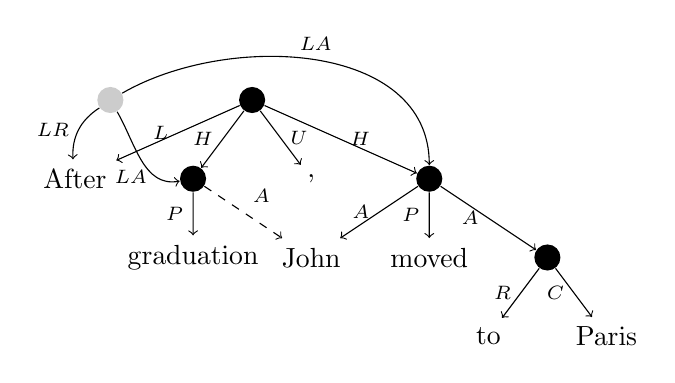
\begin{tikzpicture}[level distance=10mm, ->]
    \node (ROOT) [fill=black, circle] {}
      child {node (After) {After} edge from parent node[left] {\scriptsize $L$}}
      child {node (graduation) [fill=black, circle] {}
      {
        child {node {graduation} edge from parent node[left] {\scriptsize $P$}}
      } edge from parent node[left] {\scriptsize $H$} }
      child {node {,} edge from parent node[right] {\scriptsize $U$}}
      child {node (moved) [fill=black, circle] {}
      {
        child {node (John) {John} edge from parent node[left] {\scriptsize $A$}}
        child {node {moved} edge from parent node[left] {\scriptsize $P$}}
        child {node [fill=black, circle] {}
        {
          child {node {to} edge from parent node[left] {\scriptsize $R$}}
          child {node {Paris} edge from parent node[left] {\scriptsize $C$}}
        } edge from parent node[left] {\scriptsize $A$} }
      } edge from parent node[right] {\scriptsize $H$} }
      ;
    \draw[dashed,->] (graduation) to node [auto] {\scriptsize $A$} (John);
    \node (LKG) at (-1.8,0) [fill=black!20, circle] {};
          \draw[bend right] (LKG) to node [auto, left] {\scriptsize $LR$} (After);
          \draw (LKG) to[out=-60, in=190] node [below] {\scriptsize $LA\quad$} (graduation);
          \draw (LKG) to[out=30, in=90] node [above] {\scriptsize $LA$} (moved);
  \end{tikzpicture}
  \caption{UCCA example with linkage.}
  \label{fig:example_linkage}
\end{figure}

The linkage relation is represented by the gray node.
$LA$ is \emph{link argument}, and $LR$ is \emph{link relation}.
The relation represents the fact that the \emph{linker} ``After'' links the two parallel scenes
that are the arguments of the linkage.
Linkage relations are another source of multiple parents for a node, which we do not yet handle
in parsing and evaluation.

\paragraph{Implicit units.}

UCCA graphs may contain implicit units with no correspondent in the text.
\figref{fig:example_implicit} shows the annotation for the sentence
``A similar technique is almost impossible to apply to other crops, such as cotton, soybeans and rice.''.
The sentence was used by \citet{oepen2015semeval} to compare between different semantic
dependency schemes.
It includes a single Scene, whose main relation is ``apply'', a secondary relation ``almost impossible'', as well as two complex arguments: ``a similar technique'' and the coordinated argument ``such as cotton, soybeans, and rice.''
In addition, the scene includes an implicit argument, which represents the agent of the
``apply'' relation.

The parsing of these units is deferred to future work, as it is likely to require different methods
than those explored in this paper \cite{roth2015inducing}.

\begin{figure*}
  \centering
  \scalebox{.6}{
  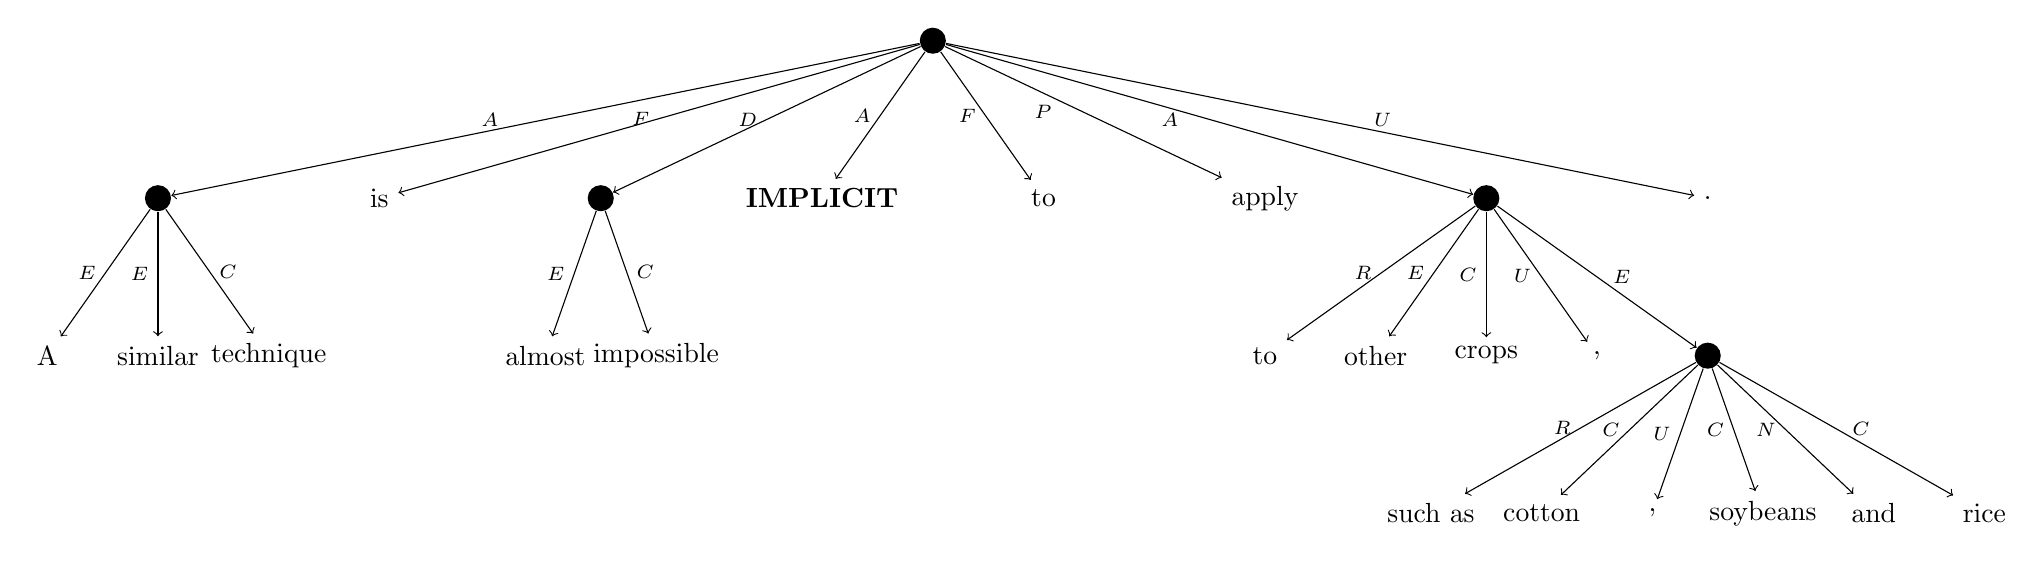
\begin{tikzpicture}[level distance=20mm, ->,
  level 1/.style={sibling distance=8em},
  level 2/.style={sibling distance=4em},
  level 3/.style={sibling distance=4em}]
    \node (ROOT) [fill=black, circle] {}
      child {node [fill=black, circle] {}
      {
        child {node {A} edge from parent node[left] {\scriptsize $E$}}
        child {node {similar} edge from parent node[left] {\scriptsize $E$}}
        child {node {technique} edge from parent node[right] {\scriptsize $C$}}
      } edge from parent node[left] {\scriptsize $A\quad$ \hspace{1mm} } }
      child {node {is} edge from parent node[left] {\scriptsize $F$}}
      child {node [fill=black, circle] {}
      {
        child {node {almost} edge from parent node[left] {\scriptsize $E$}}
        child {node {impossible} edge from parent node[right] {\scriptsize $C$}}
      } edge from parent node[left] {\scriptsize $D$} }
      child {node {\textbf{IMPLICIT}} edge from parent node[left] {\scriptsize $A$}}
      child {node {to} edge from parent node[left] {\scriptsize $F$}}
      child {node {apply} edge from parent node[left] {\scriptsize $P\quad$}}
      child {node [fill=black, circle] {}
      {
        child {node {to} edge from parent node[left] {\scriptsize $R$}}
        child {node {other} edge from parent node[left] {\scriptsize $E$}}
        child {node {crops} edge from parent node[left] {\scriptsize $C$}}
        child {node {,} edge from parent node[left] {\scriptsize $U$}}
        child {node [fill=black, circle] {}
        {
          child {node {such as} edge from parent node[left] {\scriptsize $R$}}
          child {node {cotton} edge from parent node[left] {\scriptsize $C$}}
          child {node {,} edge from parent node[left] {\scriptsize $U$}}
          child {node {soybeans} edge from parent node[left] {\scriptsize $C$}}
          child {node {and} edge from parent node[left] {\scriptsize $N$}}
          child {node {rice} edge from parent node[right] {\scriptsize $\; C$}}
        } edge from parent node[right] {\scriptsize $\; E$ \hspace{1mm} } }
      } edge from parent node[left] {\scriptsize $A\;$ \hspace{1mm} } }
      child {node {.} edge from parent node[right] {\scriptsize $\quad \quad U$}}
      ;
  \end{tikzpicture}
  }
  \caption{UCCA example with an implicit unit.}
  \label{fig:example_implicit}
\end{figure*}

\paragraph{Statistics of linkage and implicit units.}

\tabref{table:data_linkage_implicit} shows the statistics of linkage nodes and edges and
implicit nodes in the corpora.

\begin{table}[ht]
\centering
\begin{tabular}{l|ccc|c}
& \multicolumn{3}{c|}{Wiki} & 20K \\
& \small Train & \small Dev & \small Test & Leagues \\
\hline
nodes \\
\# implicit & 899 & 122 & 77 & 241 \\
\# linkage & 2956 & 263 & 359 & 376 \\
\hline
edges \\
\# linkage & 9276 & 803 & 1094 & 957
\end{tabular}
\caption{Statistics of linkage and implicit nodes in the
\textit{Wiki} and \textit{20K Leagues} UCCA corpora.
Cf. \tabref{table:data}.
}
\label{table:data_linkage_implicit}
\end{table}

\section{Rules for Extracting Linguistic Constructions}
\label{appendix:constructions}

\tabref{tab:constructions_rules} lists the rules used for extracting each linguistic
construction, used for fine-grained evaluation (see \tabref{table:constructions_results}).

\begin{table}
\scalebox{.9}{
\begin{tabular}{l|l}
Aspectual verbs & $e.P=\{\text{VERB}\} \wedge e.\ell=\text{Adverbial}$ \\
Light verbs & $e.P=\{\text{VERB}\} \wedge e.\ell=\text{Function}$ \\
MWE & $|\{e^\prime\in e.C:e^\prime.\ell=\text{Terminal}\}|>1$ \\
Pred. nouns & $\text{ADJ}\not\in e.P \wedge \text{NOUN}\in e.P \wedge {}$
 \\& $e.\ell\in\{\text{Process, State}\} \wedge {}$
 \\ \multicolumn{2}{r}{$\{e^\prime.\ell:e^\prime\in e.C\}
 	\subseteq\{\text{Center, Function, Terminal}\} \wedge {}$}
 \\& $\text{to}\not\in e.T$ \\
Pred. adjectives & $\text{ADJ}\in e.P \wedge \text{NOUN}\not\in e.P \wedge {}$
 \\& $e.\ell\in\{\text{Process, State}\} \wedge {}$
 \\ \multicolumn{2}{r}{$\{e^\prime.\ell:e^\prime\in e.C\}
 	\subseteq\{\text{Center, Function, Terminal}\} \wedge {}$}
 \\& $\text{to}\not\in e.T$ \\
Expletives & $e.T\subseteq\{\text{it, there}\} \wedge e.\ell=\text{Function}$
\end{tabular}
}
\caption{Rules for extracting linguistic constructions.
All rules are on UCCA edges. For an edge $e$ in the graph,
$e.T$ refers to the set of tokens in $e$'s yield,
and $e.P$ to their coarse parts of speech.
$e.C$ refers to the set of outgoing edges from the edge's child,
and $e.\ell$ to the edge's UCCA label.}
\label{tab:constructions_rules}
\end{table}

\section{Conversion Procedures for the Bilexical Graph and Tree Approximations}
\label{appendix:conversion}

Here we describe the algorithms used in the conversion referred to in \secref{sec:exp_setup}.

\paragraph{Notation.}
Let $L$ be the set of possible edge labels.
A UCCA graph over a sequence of tokens $w_1, \ldots, w_n$ is a directed acyclic graph
$G=(V,E, \ell)$, where $\ell:E\to L$ maps edges to labels.
For each token $w_i$ there exists a leaf (\emph{terminal}) $t_i \in V$.
A bilexical (dependency) graph over the same text consists of a set $A$ of
labeled dependency arcs $(t^\prime,l,t)$
between the terminals of $G$, where $t^\prime$ is the head, $t$ is the dependent and $l$ is
the edge label.

\paragraph{Conversion to bilexical graphs.}
Let $G=(V,E,\ell)$ be a UCCA graph with labels $\ell:E\rightarrow L$.
The conversion to a bilexical graph requires calculating the set $A$.
All non-terminals in $G$ are removed.

We define a linear order over possible edge labels $L$ (see \figref{fig:priority}).
For each node $u \in V$, denote by $h(u)$ its child with the highest-priority edge label.
Let $h^*(u)$ be the terminal reached by recursively applying $h(\cdot)$ over $u$.
For each terminal $t$, we define
\[
N(t) = \{(u,v)\in E \;|\; t=h^*(v) \wedge t \neq h^*(u) \}
\]
For each edge $(u,v)\in N(t)$, we add $h^*(u)$ as a head of $t$ in $A$,
with the label $\ell(u,v)$.
The complete conversion procedure to a bilexical graph is given in
Algorithm~\ref{alg:to_bilexical}\footnote{Note that this conversion procedure
is simpler than the head percolation procedure used for converting syntactic constituency
trees to dependency trees,
since $h(u)$ (similar to $u$'s head-containing child)
depends only on $\ell(u,h(u))$ and not on the sub-tree spanned by $u$,
because edge labels in UCCA directly express the role of the child in the parent unit, and
are thus sufficient for determining which of $u$'s children contains the head node.}.

\begin{algorithm}[ht]
 \KwData{UCCA graph ${G}=(V,E,\ell)$}
 \KwResult{set $A$ of labeled bilexical arcs}
 $A \leftarrow \emptyset$\;
 \ForEach{$t \in \mathrm{Terminals}(V)$} {
  \ForEach{$(u,v)\in N(t)$} {
   $A \leftarrow A \cup \{(h^*(u), \ell(u, v), t)\}$\;
  }
 }
 \caption{Conversion to bilexical graphs.}
 \label{alg:to_bilexical}
\end{algorithm}

\paragraph{Conversion from bilexical graphs.}
The inverse conversion introduces non-terminal nodes back into the graph.
As the distinction between low- and high-attaching nodes is lost in the
conversion, we assume that attachments are always
low-attaching.
Let $A$ be a the labeled arc set of a bilexical graph.
Iterating over the terminals in topological order according to $A$,
we add its members as terminals to graph
and create a pre-terminal parent $u_t$ for each terminal $t$,
with an edge labeled as \textit{Terminal} between them.
The parents of the pre-terminals are determined by the terminal's parent in the bilexical
graph: if $t^\prime$ is a head of $t$ in $A$, then $u_{t^\prime}$ will be a parent of $u_t$.
We add an intermediate node in between if $t$ has any dependents in $A$,
to allow adding their pre-terminals as children later.
Edge labels for the intermediate edges are determined by a rule-based function, denoted by
$\mathrm{Label}(t)$.
This procedure is given in Algorithm~\ref{alg:from_bilexical}.

\begin{algorithm}[ht]
 \KwData{list $T$ of terminals, set $A$ of labeled bilexical arcs}
 \KwResult{UCCA graph $G=(V,E,\ell)$}
 \SetKwFunction{Label}{Label}{}{}
 $V \leftarrow \emptyset$\;
 $E \leftarrow \emptyset$\;
 \ForEach{$t \in \mathrm{TopologicalSort}(T, A)$} {
  $u_t \leftarrow \mathrm{Node()}$\;
  $V \leftarrow V \cup \{u_t, t\}$\;
  $E \leftarrow E \cup \{(u_t, t)\}$\;
  $\ell(u_t,t)\leftarrow\mathit{Terminal}$\;
  \ForEach{$t^\prime\in T,l\in L$} {
   \If{$(t^\prime,l,t)\in A$} {
    \eIf{$\exists t^{\prime\prime}\in T,l^\prime\in L : (t,l^\prime,t^{\prime\prime}) \in A$} {
     $u \leftarrow \mathrm{Node()}$\;
     $V \leftarrow V \cup \{u\}$\;
     $E \leftarrow E \cup \{(u, u_t)\}$\;
     $\ell(u, u_t) \leftarrow \Label(t)$\;
    } {
     $u \leftarrow u_t$\;
    }
    $E \leftarrow E \cup \{(u_{t^\prime}, u)\}$\;
    $\ell(u_{t^\prime}, u) \leftarrow l$\;
    }
  }
 }
 
  \SetKwProg{func}{Function}{}{}
  
  \func{\Label}{
  \KwData{node $t \in T$}
  \KwResult{label $l\in L$}

   \uIf{$\mathrm{IsPunctuation}(t)$}{
    \Return \textit{Punctuation}\;
   }
   \uElseIf{$\exists t^\prime \in T : (t,\textit{ParallelScene},t^\prime)\in A$}{
    \Return \textit{ParallelScene}\;
   }
   \uElseIf{$\exists t^\prime \in T : (t,\textit{Participant},t^\prime)\in A$}{
    \Return \textit{Process}\;
   }
   \uElse{
    \Return \textit{Center}\;
   }
  }
 \caption{Conversion from bilexical graphs.}
 \label{alg:from_bilexical}
\end{algorithm}

\begin{figure}[ht]
\begin{enumerate}
\itemsep0em
\item $C$ (\textit{Center})
\item $N$ (\textit{Connector})
\item $H$ (\textit{ParallelScene})
\item $P$ \textit{Process})
\item $S$ (\textit{State})
\item $A$ (\textit{Participant})
\item $D$ (\textit{Adverbial})
\item $T$ (\textit{Time})
\item $E$ (\textit{Elaborator})
\item $R$ (\textit{Relator})
\item $F$ (\textit{Function})
\item $L$ (\textit{Linker})
\item $LR$ (\textit{LinkRelation})
\item $LA$ (\textit{LinkArgument})
\item $G$ (\textit{Ground})
\item $\mathit{Terminal}$ (\textit{Terminal})
\item $U$ (\textit{Punctuation})
\end{enumerate}
\caption{Priority order of edge labels, used in Algorithm~\ref{alg:to_bilexical}.}
\label{fig:priority}
\end{figure}

\paragraph{Conversion to trees.}

To convert a UCCA graph to a tree, we simply remove the remote edges.
Converting the sentence in \figref{fig:graduation}
results in the tree given in \figref{fig:con_example}.

\begin{figure}[ht]
  \centering
  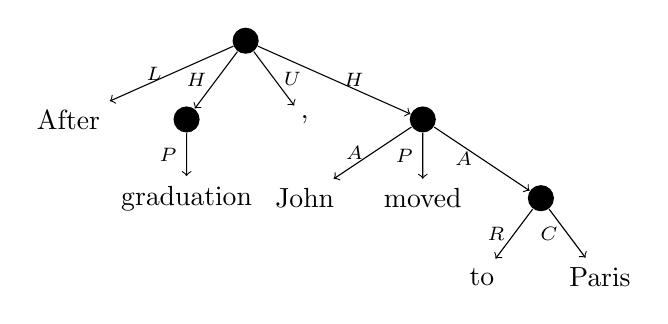
\begin{tikzpicture}[level distance=10mm, ->]
    \node (ROOT) [fill=black, circle] {}
      child {node (After) {After} edge from parent node[left] {\scriptsize $L$}}
      child {node (graduation) [fill=black, circle] {}
      {
        child {node {graduation} edge from parent node[left] {\scriptsize $P$}}
      } edge from parent node[left] {\scriptsize $H$} }
      child {node {,} edge from parent node[right] {\scriptsize $U$}}
      child {node (moved) [fill=black, circle] {}
      {
        child {node (John) {John} edge from parent node[left] {\scriptsize $A$}}
        child {node {moved} edge from parent node[left] {\scriptsize $P$}}
        child {node [fill=black, circle] {}
        {
          child {node {to} edge from parent node[left] {\scriptsize $R$}}
          child {node {Paris} edge from parent node[left] {\scriptsize $C$}}
        } edge from parent node[left] {\scriptsize $A$} }
      } edge from parent node[right] {\scriptsize $H$} }
      ;
  \end{tikzpicture}
  \caption{Tree approximation for the UCCA graph in \figref{fig:graduation}.}
  \label{fig:con_example}
\end{figure}

To convert a UCCA graph to a bilexical tree, we first convert it to a bilexical graph, and then
remove the remote edges.
The corresponding dependency tree is given in \figref{fig:dep_example}.

\begin{figure}[ht]
\centering
\begin{dependency}[theme = simple]
\begin{deptext}[column sep=.7em,ampersand replacement=\^]
After \^ graduation \^ , \^ John \^ moved \^ to \^ Paris \\
\end{deptext}
\depedge{2}{1}{L}
\depedge{2}{3}{U}
\depedge{5}{4}{A}
\depedge{2}{5}{H}
\depedge{7}{6}{R}
\depedge{5}{7}{A}
\end{dependency}
  \caption{Bilexical tree approximation for the UCCA graph in \figref{fig:graduation}.}
  \label{fig:dep_example}
\end{figure}

\end{document}
